La metodología propuesta incluye la recolección de datos mediante web scraping de plataformas inmobiliarias, su enriquecimiento con información de fuentes abiertas como mapas de servicios y boletines de seguridad, y el entrenamiento de modelos predictivos utilizando técnicas de machine learning. Los pasos clave del proceso se ilustran en la Figura \ref{fig:metodologia}.

\begin{figure}
    \centering
    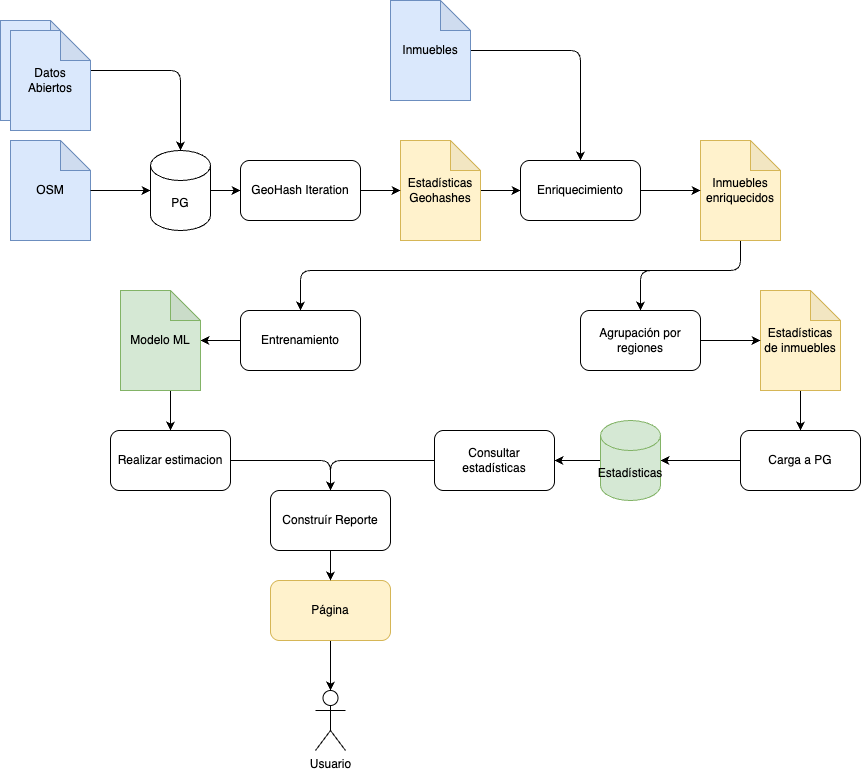
\includegraphics[width=0.85\linewidth]{Images/metodologia.png}
    \caption{Proceso general de la metodología}
    \label{fig:metodologia}
\end{figure}

\subsection*{Recolección de Datos a través de Web Scraping}
Esta etapa consistirá en la extracción de datos de varios portales inmobiliarios utilizando una aplicación desarrollada en Java. Los datos recopilados incluirán características de las propiedades como ubicación, área construida, número de habitaciones, baños y precios.

\begin{itemize}
    \item \textbf{Herramientas}: Java para la implementación de la aplicación de \textit{web scraping}, utilizando bibliotecas como \texttt{Jsoup} o \texttt{HtmlUnit} para la extracción de datos.
    \item \textbf{Validación}: Asegurar la correcta extracción de los datos mediante la limpieza inicial y la eliminación de duplicados o datos incompletos.
\end{itemize}

\subsection*{Limpieza y Preprocesamiento de Datos (en Python)}
Una vez recolectados los datos con la aplicación en Java, se exportarán a un formato manejable (como CSV o JSON) y se realizará la limpieza y preprocesamiento en Python. Esto incluye la gestión de valores faltantes, normalización de variables y eliminación de \textit{outliers}.

\begin{itemize}
    \item \textbf{Herramientas}: \textit{Pandas} y \textit{NumPy} en Python para manipulación de datos, junto con \textit{scikit-learn} para el preprocesamiento.
    \item \textbf{Validación}: Verificar que los datos estén correctamente preparados para ser utilizados en los modelos predictivos.
\end{itemize}

\subsection*{Enriquecimiento de los Datos con Fuentes Externas (en Python)}
En esta fase, los datos se enriquecerán con información externa como indicadores de seguridad, proximidad a sitios de interés (parques, colegios, hospitales) y otros factores que influyan en los precios de las viviendas.

\begin{itemize}
    \item \textbf{Herramientas}: APIs de datos abiertos, \textit{Geopandas} para el análisis geoespacial, y \textit{Pandas} para la integración de datos.
    \item \textbf{Validación}: Comprobar que la integración de los datos externos sea precisa y que los datos estén listos para alimentar los modelos predictivos.
\end{itemize}

\subsection*{Desarrollo de Modelos Predictivos (en Python)}
Se desarrollarán varios modelos de \textit{machine learning} en Python, como regresión lineal, \textit{random forest}, y redes neuronales, para comparar su rendimiento en la predicción de precios de las viviendas.

\begin{itemize}
    \item \textbf{Herramientas}: \textit{scikit-learn} para la implementación de modelos de \textit{machine learning}, y \textit{TensorFlow} o \textit{Keras} para redes neuronales.
    \item \textbf{Validación}: Validación cruzada para evaluar el rendimiento y garantizar que los modelos no estén sobreajustados a los datos.
\end{itemize}

\subsection*{Evaluación y Selección del Mejor Modelo (en Python)}
Se seleccionará el mejor modelo basado en métricas de evaluación como el \textit{Mean Absolute Error (MAE)}, \textit{Mean Squared Error (MSE)} y el \textit{Coeficiente de Determinación (R²)}.

\begin{itemize}
    \item \textbf{Herramientas}: \textit{scikit-learn} para las métricas de evaluación.
    \item \textbf{Validación}: Selección del modelo con mejor rendimiento en términos de precisión y capacidad de generalización.
\end{itemize}

\subsection*{Visualización y Análisis de Resultados (en Python)}
Se realizarán visualizaciones de los resultados obtenidos, mostrando los factores más influyentes en la predicción de precios y generando gráficos que ilustren la distribución de los errores. Además, se crearán mapas que relacionen la ubicación geográfica con los precios de las propiedades.

\begin{itemize}
    \item \textbf{Herramientas}: \textit{Matplotlib} y \textit{Seaborn} para visualización de datos, \textit{Geopandas} para mapas.
    \item \textbf{Validación}: Garantizar que las visualizaciones sean claras y útiles para interpretar los resultados del modelo.
\end{itemize}

\subsection*{Documentación y Presentación del Proyecto}
Se documentará todo el proceso, detallando desde la recolección de datos con Java hasta la evaluación y selección del modelo en Python. La documentación será clave para la redacción del informe final del proyecto de grado.

\begin{itemize}
    \item \textbf{Herramientas}: \textit{LaTeX} o herramientas de procesamiento de texto.
    \item \textbf{Validación}: Revisión final de toda la documentación y presentación para asegurar que esté completa y bien estructurada.
\end{itemize}
